% This file was converted to LaTeX by Writer2LaTeX ver. 1.6.1
% see http://writer2latex.sourceforge.net for more info
\documentclass[a4paper,dvipdfmx]{jarticle}
\usepackage[latin1]{inputenc}
\usepackage{amsmath}
\usepackage{amssymb,amsfonts,textcomp}
\usepackage[T1]{fontenc}
\usepackage[english]{babel}
\usepackage{color}
\usepackage{array}
\usepackage{supertabular}
\usepackage{hhline}
\usepackage{hyperref}
\usepackage{pxjahyper}
\hypersetup{dvipdfmx, colorlinks=true, linkcolor=blue, citecolor=blue, filecolor=blue, urlcolor=blue, pdftitle=子どもIT未来塾 第6回, pdfauthor=, pdfsubject=, pdfkeywords=}
\usepackage[dvipdfmx]{graphicx}
\graphicspath{%
{./text06-img/}%
}
% Outline numbering
\setcounter{secnumdepth}{3}
\renewcommand\thesection{\arabic{section}}
\renewcommand\thesubsection{\arabic{section}.\arabic{subsection}}
\renewcommand\thesubsubsection{\arabic{section}.\arabic{subsection}.\arabic{subsubsection}}
% Page layout (geometry)
\setlength\voffset{-1in}
\setlength\hoffset{-1in}
\setlength\topmargin{2cm}
\setlength\oddsidemargin{2cm}
\setlength\textheight{24.770668cm}
\setlength\textwidth{17.006cm}
\setlength\footskip{26.144882pt}
\setlength\headheight{0cm}
\setlength\headsep{0cm}
% Footnote rule
\setlength{\skip\footins}{0.12cm}
\renewcommand\footnoterule{\vspace*{-0.018cm}\setlength\leftskip{0pt}\setlength\rightskip{0pt plus 1fil}\noindent\textcolor{black}{\rule{0.25\columnwidth}{0.018cm}}\vspace*{0.102cm}}
% Pages styles
\makeatletter
\newcommand\ps@Standard{
  \renewcommand\@oddhead{}
  \renewcommand\@evenhead{}
  \renewcommand\@oddfoot{2019年8月25日\hfill 子どもIT未来塾 第6回\hfill Page \thepage{}\ of ?}
  \renewcommand\@evenfoot{\@oddfoot}
  \renewcommand\thepage{\arabic{page}}
}
\newcommand\ps@FirstPage{
  \renewcommand\@oddhead{}
  \renewcommand\@evenhead{}
  \renewcommand\@oddfoot{}
  \renewcommand\@evenfoot{\@oddfoot}
  \renewcommand\thepage{\arabic{page}}
}
\makeatother
\pagestyle{Standard}
\setlength\tabcolsep{1mm}
\renewcommand\arraystretch{1.3}
% List styles
\newcommand\liststyleLi{%
\renewcommand\theenumi{\arabic{enumi}}
\renewcommand\theenumii{\arabic{enumii}}
\renewcommand\theenumiii{\arabic{enumiii}}
\renewcommand\theenumiv{\arabic{enumiv}}
\renewcommand\labelenumi{\theenumi.}
\renewcommand\labelenumii{\theenumii.}
\renewcommand\labelenumiii{\theenumiii.}
\renewcommand\labelenumiv{\theenumiv.}
}
\newcommand\liststyleLii{%
\renewcommand\theenumi{\arabic{enumi}}
\renewcommand\theenumii{\arabic{enumii}}
\renewcommand\theenumiii{\arabic{enumiii}}
\renewcommand\theenumiv{\arabic{enumiv}}
\renewcommand\labelenumi{\theenumi.}
\renewcommand\labelenumii{\theenumii.}
\renewcommand\labelenumiii{\theenumiii.}
\renewcommand\labelenumiv{\theenumiv.}
}
\newcommand\liststyleLiii{%
\renewcommand\theenumi{\arabic{enumi}}
\renewcommand\theenumii{\arabic{enumii}}
\renewcommand\theenumiii{\arabic{enumiii}}
\renewcommand\theenumiv{\arabic{enumiv}}
\renewcommand\labelenumi{\theenumi.}
\renewcommand\labelenumii{\theenumii.}
\renewcommand\labelenumiii{\theenumiii.}
\renewcommand\labelenumiv{\theenumiv.}
}
\newcommand\liststyleLiv{%
\renewcommand\theenumi{\arabic{enumi}}
\renewcommand\theenumii{\arabic{enumii}}
\renewcommand\theenumiii{\arabic{enumiii}}
\renewcommand\theenumiv{\arabic{enumiv}}
\renewcommand\labelenumi{\theenumi.}
\renewcommand\labelenumii{\theenumii.}
\renewcommand\labelenumiii{\theenumiii.}
\renewcommand\labelenumiv{\theenumiv.}
}
\newcommand\liststyleLv{%
\renewcommand\labelitemi{{\textbullet}}
\renewcommand\labelitemii{${\circ}$}
\renewcommand\labelitemiii{${\blacksquare}$}
\renewcommand\labelitemiv{{\textbullet}}
}
\newcommand\liststyleLvi{%
\renewcommand\labelitemi{{\textbullet}}
\renewcommand\labelitemii{${\circ}$}
\renewcommand\labelitemiii{${\blacksquare}$}
\renewcommand\labelitemiv{{\textbullet}}
}
\newcommand\liststyleLvii{%
\renewcommand\theenumi{\arabic{enumi}}
\renewcommand\theenumii{\arabic{enumii}}
\renewcommand\theenumiii{\arabic{enumiii}}
\renewcommand\theenumiv{\arabic{enumiv}}
\renewcommand\labelenumi{\theenumi.}
\renewcommand\labelenumii{\theenumii.}
\renewcommand\labelenumiii{\theenumiii.}
\renewcommand\labelenumiv{\theenumiv.}
}
\newcommand\liststyleLviii{%
\renewcommand\labelitemi{{\textbullet}}
\renewcommand\labelitemii{${\circ}$}
\renewcommand\labelitemiii{${\blacksquare}$}
\renewcommand\labelitemiv{{\textbullet}}
}
\newcommand\liststyleLix{%
\renewcommand\theenumi{\arabic{enumi}}
\renewcommand\theenumii{\arabic{enumii}}
\renewcommand\theenumiii{\arabic{enumiii}}
\renewcommand\theenumiv{\arabic{enumiv}}
\renewcommand\labelenumi{\theenumi.}
\renewcommand\labelenumii{\theenumii.}
\renewcommand\labelenumiii{\theenumiii.}
\renewcommand\labelenumiv{\theenumiv.}
}
\newcommand\liststyleLx{%
\renewcommand\theenumi{\arabic{enumi}}
\renewcommand\theenumii{\arabic{enumii}}
\renewcommand\theenumiii{\arabic{enumiii}}
\renewcommand\theenumiv{\arabic{enumiv}}
\renewcommand\labelenumi{\theenumi.}
\renewcommand\labelenumii{\theenumii.}
\renewcommand\labelenumiii{\theenumiii.}
\renewcommand\labelenumiv{\theenumiv.}
}
\newcommand\liststyleLxi{%
\renewcommand\theenumi{\arabic{enumi}}
\renewcommand\theenumii{\arabic{enumii}}
\renewcommand\theenumiii{\arabic{enumiii}}
\renewcommand\theenumiv{\arabic{enumiv}}
\renewcommand\labelenumi{\theenumi.}
\renewcommand\labelenumii{\theenumii.}
\renewcommand\labelenumiii{\theenumiii.}
\renewcommand\labelenumiv{\theenumiv.}
}
\newcommand\liststyleLxii{%
\renewcommand\theenumi{\arabic{enumi}}
\renewcommand\theenumii{\arabic{enumii}}
\renewcommand\theenumiii{\arabic{enumiii}}
\renewcommand\theenumiv{\arabic{enumiv}}
\renewcommand\labelenumi{\theenumi.}
\renewcommand\labelenumii{\theenumii.}
\renewcommand\labelenumiii{\theenumiii.}
\renewcommand\labelenumiv{\theenumiv.}
}
\newcommand\liststyleLxiii{%
\renewcommand\theenumi{\arabic{enumi}}
\renewcommand\theenumii{\arabic{enumii}}
\renewcommand\theenumiii{\arabic{enumiii}}
\renewcommand\theenumiv{\arabic{enumiv}}
\renewcommand\labelenumi{\theenumi.}
\renewcommand\labelenumii{\theenumii.}
\renewcommand\labelenumiii{\theenumiii.}
\renewcommand\labelenumiv{\theenumiv.}
}
\newcommand\liststyleLxiv{%
\renewcommand\theenumi{\arabic{enumi}}
\renewcommand\theenumii{\arabic{enumii}}
\renewcommand\theenumiii{\arabic{enumiii}}
\renewcommand\theenumiv{\arabic{enumiv}}
\renewcommand\labelenumi{\theenumi.}
\renewcommand\labelenumii{\theenumii.}
\renewcommand\labelenumiii{\theenumiii.}
\renewcommand\labelenumiv{\theenumiv.}
}
\newcommand\liststyleLxv{%
\renewcommand\theenumi{\arabic{enumi}}
\renewcommand\theenumii{\arabic{enumii}}
\renewcommand\theenumiii{\arabic{enumiii}}
\renewcommand\theenumiv{\arabic{enumiv}}
\renewcommand\labelenumi{\theenumi.}
\renewcommand\labelenumii{\theenumii.}
\renewcommand\labelenumiii{\theenumiii.}
\renewcommand\labelenumiv{\theenumiv.}
}
\newcommand\liststyleLxvi{%
\renewcommand\labelitemi{{\textbullet}}
\renewcommand\labelitemii{${\circ}$}
\renewcommand\labelitemiii{${\blacksquare}$}
\renewcommand\labelitemiv{{\textbullet}}
}
\newcommand\liststyleLxvii{%
\renewcommand\theenumi{\arabic{enumi}}
\renewcommand\theenumii{\arabic{enumii}}
\renewcommand\theenumiii{\arabic{enumiii}}
\renewcommand\theenumiv{\arabic{enumiv}}
\renewcommand\labelenumi{\theenumi.}
\renewcommand\labelenumii{\theenumii.}
\renewcommand\labelenumiii{\theenumiii.}
\renewcommand\labelenumiv{\theenumiv.}
}
\newcommand\liststyleLxviii{%
\renewcommand\labelitemi{{\textbullet}}
\renewcommand\labelitemii{${\circ}$}
\renewcommand\labelitemiii{${\blacksquare}$}
\renewcommand\labelitemiv{{\textbullet}}
}
\newcommand\liststyleLxix{%
\renewcommand\labelitemi{{\textbullet}}
\renewcommand\labelitemii{${\circ}$}
\renewcommand\labelitemiii{${\blacksquare}$}
\renewcommand\labelitemiv{{\textbullet}}
}
\newcommand\liststyleLxx{%
\renewcommand\labelitemi{{\textbullet}}
\renewcommand\labelitemii{${\circ}$}
\renewcommand\labelitemiii{${\blacksquare}$}
\renewcommand\labelitemiv{{\textbullet}}
}
% Non-floating captions
\makeatletter
\newcommand\captionof[2]{\def\@captype{#1}\caption{#2}}
\makeatother
\newcounter{List}
\renewcommand\theList{\arabic{List}}
\title{子どもIT未来塾 第6回}
\author{}
\date{2021-09-22}
\begin{document}
\clearpage\setcounter{page}{1}\pagestyle{Standard}
\thispagestyle{FirstPage}

\bigskip

\clearpage\section{音声合成}
%\begin{figure}
\centering
\begin{minipage}{17.369cm}
\clearpage\setcounter{page}{1}\pagestyle{Standard}
\thispagestyle{FirstPage}
{\centering\bfseries
子どもIT未来塾 第6回
\par}

{\centering\bfseries
音声合成と音声認識
\par}

{\centering\bfseries
2019年8月25日
\par}

{\centering\bfseries
\ 奥山 祐市\newline
荒川麻衣子\newline
新明洋平\newline
小堺美咲
\par}
\end{minipage}
%\end{figure}
{\selectlanguage{english}
音声合成とは何でしょう。それは、人間の声を人工的に機械で作り出すことです。みなさんが目にするもので言えば、例えばソフトバンクが制作するpepper(\figurename~\ref{seq:refIllustration0})というロボットがあります。}

\captionof{figure}[pepper (softbank)]{ 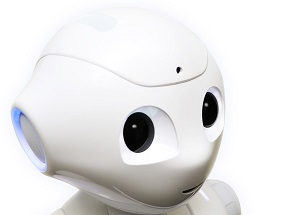
\includegraphics[width=7.938cm,height=5.689cm]{text06-img/text06-img001.jpg}
\newline
pepper (softbank)}
\label{seq:refIllustration0}


{\selectlanguage{english}
これは声を出して利用者とコミュニケーションを取ります。pepperから声が出るのは、中に人間が入っているわけではありません。読み上げたい文章があったとき、それに\textcolor{black}{マッチした}音声を生成し、スピーカーから発しているのです。}

{\selectlanguage{english}
今回は音声を合成するために、OpenJTalkと呼ばれる音声合成のためのソフトウェアを使います。OpenJTalkは、読み上げたい文章と、ひらがなごとの音(厳密にはもう少し\textcolor{black}{多種}の音)を入力し、対応する音声ファイルを出力します(\figurename~\ref{seq:refIllustration1})。}



%\begin{figure}
\centering
\caption[OpenJTalkの入出力]{[Warning: Draw object ignored]OpenJTalkの入出力}
\label{seq:refIllustration1}

%\end{figure}
{\bfseries
問題6-1}

\liststyleLi
\begin{enumerate}
\item {\selectlanguage{english}
音声合成とはなんですか。20字以内で説明してください。}


\bigskip

\begin{enumerate}
\item \begin{enumerate}
\item[] {\raggedleft\ttfamily\bfseries
答え.\_\_\_\_\_\_\_\_\_\_\_\_\_\_\_\_\_\_\_\_\_\_\_\_\_\_\_\_\_\_\_\_\_\_\_\_\_\_\_\_\_\_\_\_\_\_\_\_\_\_\_\_\_\_\_\_\_\_\_\_\_\_\_\_
\par}
\end{enumerate}
\end{enumerate}
\item {\selectlanguage{english}
音声合成をするにはパソコンに何を準備する必要がありますか。3つ挙げてください。}
\end{enumerate}
\liststyleLii
\begin{enumerate}
\item[] 
\bigskip

\begin{enumerate}
\item \begin{enumerate}
\item[] {\raggedleft\ttfamily\bfseries
答え.\_\_\_\_\_\_\_\_\_\_\_\_\_\_\_\_\_\_\_\_\_\_\_\_\_\_\_\_\_\_\_\_\_\_\_\_\_\_\_\_\_\_\_\_\_\_\_\_\_\_\_\_\_\_\_\_\_\_\_\_\_\_\_\_
\par}
\end{enumerate}
\end{enumerate}
\end{enumerate}

\bigskip

\clearpage\section{音声認識}
{\selectlanguage{english}
音声認識は、音声合成とは逆に、文章を読み上げている音声ファイルからその文章を予想するものです。例えばGoogleのGoogle
Homeはまさにこれです。「1時間後に起こして」と声を発すると、内部でそれが文字列に変換されます。その後その文字列を解析してアラームを設定します。}

{\selectlanguage{english}
音声認識のためのソフトウェアとしてJuliusというものを使います。入力は音声で出力は文字列になります(\figurename~\ref{seq:refIllustration2})。}



%\begin{figure}
\centering
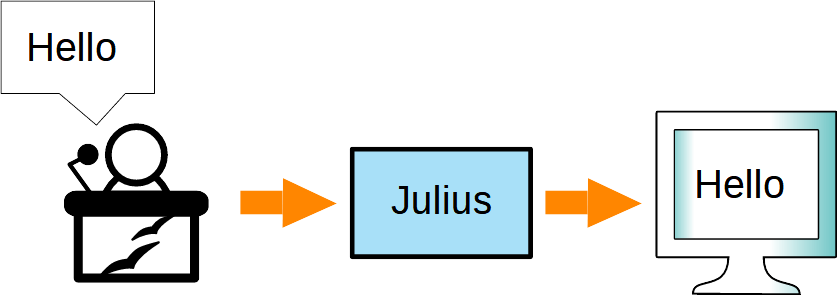
\includegraphics[width=17.006cm,height=6.006cm]{text06-img/text06-img002.png}
\caption[Juliusの入出力]{\newline
Juliusの入出力}
\label{seq:refIllustration2}

%\end{figure}
{\selectlanguage{english}
問題6-2}

\liststyleLiii
\begin{enumerate}
\item {\selectlanguage{english}
音声認識とはなんですか。50字以内で説明してください。}
\end{enumerate}
\liststyleLii
\begin{enumerate}
\item[] 
\bigskip

\begin{enumerate}
\item \begin{enumerate}
\item[] {\raggedleft\ttfamily\bfseries
答え.\_\_\_\_\_\_\_\_\_\_\_\_\_\_\_\_\_\_\_\_\_\_\_\_\_\_\_\_\_\_\_\_\_\_\_\_\_\_\_\_\_\_\_\_\_\_\_\_\_\_\_\_\_\_\_\_\_\_\_\_\_\_\_\_
\par}
\end{enumerate}
\end{enumerate}
\end{enumerate}

\bigskip

\section{ヘッドセットの使い方}
{\selectlanguage{english}
演習の前に、ヘッドセットの設定をしましょう。ヘッドセットとは、コンピュータなどから音声を出力するためのヘッドフォンと、コンピュータなどに音声を入力するためのマイクが一体型になったものです。}

{\selectlanguage{english}
まずはラズベリーパイの電源を入れる前に、ヘッドセットとラズベリーパイをつないでおきます。}

{\centering 
\captionof{figure}[つなげかた]{
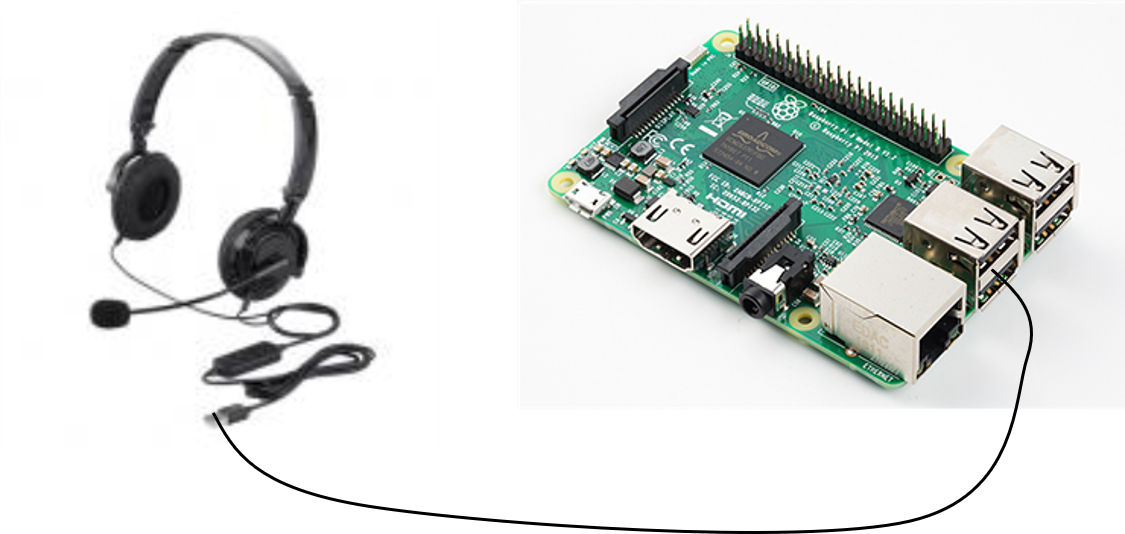
\includegraphics[width=10.261cm,height=4.87cm]{text06-img/text06-img003.png} \newline
つなげかた}
\par}
{\selectlanguage{english}
ヘッドセットの出力音量はコントローラーかディスプレイで調整できます。}

{\centering 
\captionof{figure}[ヘッドセットのコントローラーの使い方]{
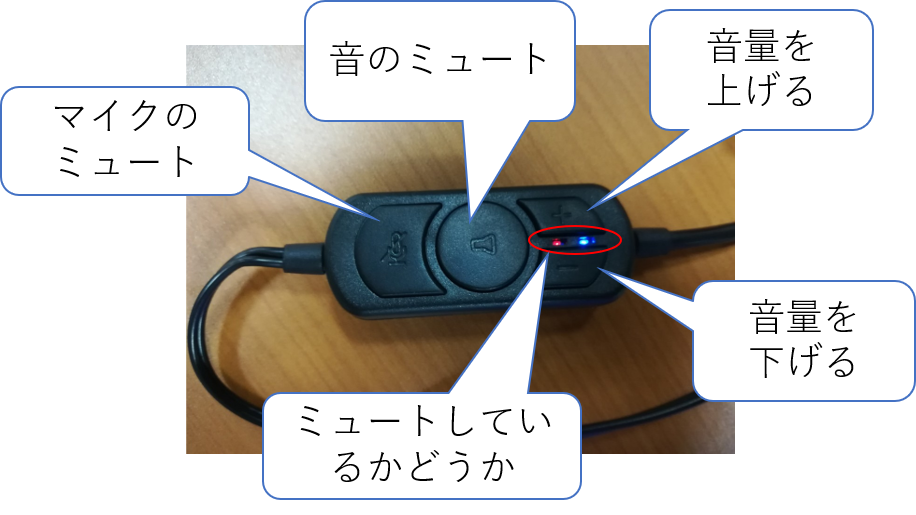
\includegraphics[width=10.188cm,height=5.727cm]{text06-img/text06-img004.png} \newline
ヘッドセットのコントローラーの使い方}
\par}
{\selectlanguage{english}
一番左のボタンでマイクのミュートを切りかえることができます。ミュートとは音を消すことです。マイクがミュートしているときは赤色のLEDが光っています。マイクを使うときはミュートを解除して、赤色のLEDが光っていないようにしましょう。真ん中のボタンは音のミュートです。音が聞こえないときはここを押してみましょう。右側のボタンは''+''で音量を上げる、{}''-''で音量を下げることができます。}

{\selectlanguage{english}
マイクの音量はディスプレイからも設定できます。}



%\begin{figure}
\centering
\caption[使う音声デバイスの選択と設定]{
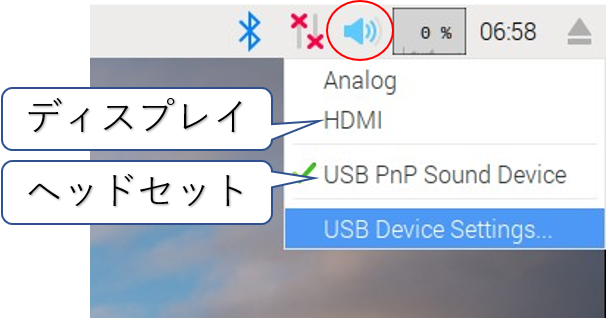
\includegraphics[width=10.262cm,height=5.385cm]{text06-img/text06-img005.png} \newline
使う音声デバイスの選択と設定}
\label{seq:refIllustration5}

%\end{figure}
{\selectlanguage{english}
ディスプレイの右上にある音マークを右クリックしてみましょう。使うことのできるデバイスが表示されます。HDMIとはディスプレイのことです。これを左クリックするとディスプレイから音を出すことができます。教室ではヘッドセットを使いますが、おうちではお父さんやお母さんにいいよと言われたら、ディスプレイやテレビから出力することもできます。USB
PnP Sound
Deviceはヘッドセットのことです。ヘッドセットを使うときはこちらを左クリックします。}

{\selectlanguage{english}
音量を変えるときは一番下のUSB Device
Settings...を左クリックします。}

\begin{center}
\tablefirsthead{}
\tablehead{}
\tabletail{}
\tablelasttail{}
\begin{supertabular}{|l|l|l|}
\hline
{
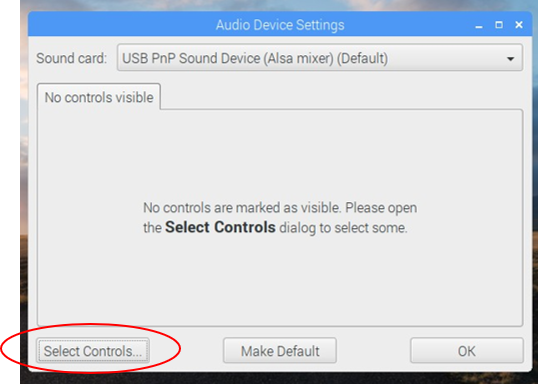
\includegraphics[width=5.475cm,height=3.907cm]{text06-img/text06-img006.png} \newline
画面の右上の音マークから USB Device Settings...
をクリックしたところ。マイクの入力音量を調節するには、Select
Controls をクリックする。}
 &
{
		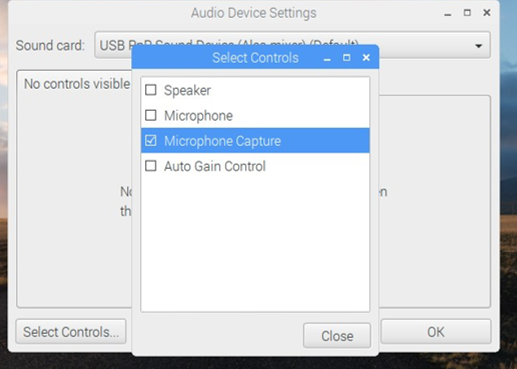
\includegraphics[width=5.475cm,height=3.907cm]{text06-img/text06-img007.png} \newline
配布したヘッドセットのマイク設定をするために、「Microphone
Capture」 をクリック。}

 & %\centering
{
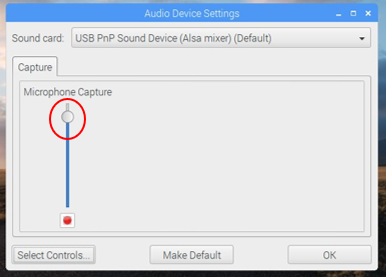
\includegraphics[width=5.475cm,height=3.928cm]{text06-img/text06-img008.png} \newline
バーを上げ下げしてマイクの音量を調節する。}
\label{seq:refIllustration8}
\\\hline
\end{supertabular}
\end{center}
{\selectlanguage{english}
左下のSelect
Controlsをクリックすると、真ん中の画面が出てきます。Microphone
Captureをクリックしチェックを付けて画面を閉じます。すると右の画面のように音量調節バーが出ます。丸いつまみを上下に動かすことで音量を調節することができます。}

{\selectlanguage{english}
教室ではヘッドセットで音を聞き、ヘッドセットのマイクで音声を入力するので、図\ref{seq:refIllustration5}
のように USB PnP Sound Device
を選択し、図\ref{seq:refIllustration8}のようにマイクの入力音量を大きめにしておきましょう。}

\section[OpenJTalk]{OpenJTalk}
{\selectlanguage{english}
ここでは音声合成ソフトウェアOpenJTalkの紹介をします。まずは使ってみましょう。}

\subsection[文を読み上げてもらう]{文を読み上げてもらう}
{\selectlanguage{english}
文を読み上げるHSPプログラムを紹介します。openjtalk.hsp
をHSPスクリプトエディタで開いてください。openjtalk.hsp
は /home/pi/ome/06/ の中にあります。}

\begin{minipage}{17.006cm}
[Warning: Draw object ignored]{\ttfamily\bfseries
\#include {\textquotedbl}hsp3dish.as{\textquotedbl}}

\begin{minipage}{15.863cm}
[Warning: Draw object ignored]{\ttfamily\bfseries
jtload {\textquotedbl}子どもIT未来塾{\textquotedbl},
0\ \ \textcolor[rgb]{0.0,0.0,0.6}{;音声ファイルを出力し、読み込む}}

{\ttfamily\bfseries
mmplay
0\ \ \ \ \ \ \ \ \textcolor[rgb]{0.0,0.0,0.6}{;音声ファイルを再生する}}
\end{minipage}{\ttfamily\bfseries
\#include {\textquotedbl}jtalk.as{\textquotedbl}}


\bigskip

{\ttfamily\bfseries
redraw 0}

{\ttfamily\bfseries
mes {\textquotedbl}発話開始{\textquotedbl}}

{\ttfamily\bfseries
mes {\textquotedbl}「子どもIT未来塾」{\textquotedbl}}

{\ttfamily\bfseries
redraw 1}


\bigskip


\bigskip

{\ttfamily\bfseries
stop}

{\upshape
リスト \stepcounter{List}{\theList}: openjtalk.hsp}
\end{minipage}

{\selectlanguage{english}
2行目}

{\ttfamily\bfseries
\#include ``jtalk.as''}

{\selectlanguage{english}
で、openjtalkをHSPで使うのに必要な設定が行われます。この行によって、後に説明する
jtload 命令と setvoice
命令が使えるようになります。}

{\selectlanguage{english}
4行目から7行目までは復習です。mes命令で文字を表示させています。}

{\selectlanguage{english}
9行目からが新しい命令です。}

{\ttfamily\bfseries
jtload {\textquotedbl}子どもIT未来塾{\textquotedbl}, 0}

{\selectlanguage{english}
で、0番のバッファに ``子どもIT未来塾''
と読ませた音声ファイルがロードされます。
画像を配置するときや、I2Cを使うときと同じような仕組みです。より一般的に書くと、jtload命令は}

{\ttfamily\bfseries
jtload {\textless}読み上げ文字列{\textgreater},
{\textless}バッファ番号{\textgreater}}

{\selectlanguage{english}
となります。}

{\selectlanguage{english}
10行目}

{\ttfamily\bfseries
mmplay 0}

{\selectlanguage{english}
で、0番のバッファ(今ロードしたバッファ)を再生します。より一般的に書くと、}

{\ttfamily\bfseries
mmplay {\textless}再生するバッファ番号{\textgreater}}

{\selectlanguage{english}
となります。この命令は再生開始後すぐに次の命令を実行するので、複数の音声を順番に再生したいときはwait命令を入れるなどの工夫が必要になります。}


\bigskip

\subsubsection{問題6-3}
\liststyleLiv
\begin{enumerate}
\item {\selectlanguage{english}
「本日は青天なり」と読み上げるようにプログラムを書き変えて、sunny.hspという名前で/home/pi/ome/06/に保存し、実行しましょう。\newline
ヒント:jtload {\textquotedbl}子どもIT未来塾{\textquotedbl},
0をかきかえます。\newline
${\square}\leftarrow
できたらチェックしましょう。$}
\item {\selectlanguage{english}
時間があったらやりましょう。\newline
好きな言葉を読み上げさせましょう。\newline
${\square}\leftarrow
できたらチェックしましょう。$}
\end{enumerate}
\subsection[声音を変えてみる]{声音を変えてみる}
{\selectlanguage{english}
ところで、人間の声は人によって高い声だったり低い声だったり違いますよね。Openjtalkでは文章を読ませるときの声音を指定することができます。声音はhtsvoiceというファイルフォーマットによって定められおり、setvoice
命令で指定することができます。}

{\ttfamily\bfseries
setvoice {\textless}声音ファイル{\textgreater}}


\bigskip

{\selectlanguage{english}
{\textless}声音ファイル{\textgreater}は、/home/pi/ome/bin/openjtalk/voices/
以下のパスを書きます。}

{\selectlanguage{english}
みなさんのRaspberry
Piにはいくつかの声音ファイルがすでにダウンロードされています。
/home/pi/ome/bin/openjtalk/voicesを見てみてください。女声として}

\liststyleLv
\begin{itemize}
\item {\selectlanguage{english}
tonaeyoe/tonaeyoe.htsvoice}
\item {\selectlanguage{english}
htsvoice-tohoku-f01/tohoku-f01-neutral.htsvoice}
\item {\selectlanguage{english}
htsvoice-tohoku-f01/tohoku-f01-angry.htsvoice}
\item {\selectlanguage{english}
htsvoice-tohoku-f01/tohoku-f01-happy.htsvoice}
\item {\selectlanguage{english}
htsvoice-tohoku-f01/tohoku-f01-sad.htsvoice}
\end{itemize}
{\selectlanguage{english}
を、男声として}

\liststyleLvi
\begin{itemize}
\item {\selectlanguage{english}
gigarakan/gigarakan.htsvoice}
\end{itemize}
{\selectlanguage{english}
を利用できます。例を示します。/home/pi/ome/06/voice.hsp
をHSPスクリプトエディタで開いてみましょう。}

\begin{minipage}{17.006cm}
[Warning: Draw object ignored]{\ttfamily\bfseries
\#include {\textquotedbl}hsp3dish.as{\textquotedbl}}

\begin{minipage}{16.665cm}
[Warning: Draw object ignored]{\ttfamily\bfseries
setvoice
{\textquotedbl}htsvoice-tohoku-f01/tohoku-f01-sad.htsvoice{\textquotedbl}\ \ \textcolor[rgb]{0.0,0.0,0.6}{;音声ファイル指定}}

{\ttfamily\bfseries
jtload {\textquotedbl}子どもIT未来塾{\textquotedbl},
0\ \ \textcolor[rgb]{0.0,0.0,0.6}{;音声ファイル生成と読み込み}}

{\ttfamily\bfseries
mmplay 0\ \ \ \ \ \ \ \ \textcolor[rgb]{0.0,0.0,0.6}{;音声ファイルの再生}}
\end{minipage}{\ttfamily\bfseries
\#include {\textquotedbl}jtalk.as{\textquotedbl}}


\bigskip

{\ttfamily\bfseries
redraw 0}

{\ttfamily\bfseries
mes {\textquotedbl}発話開始{\textquotedbl}}

{\ttfamily\bfseries
mes {\textquotedbl}「子どもIT未来塾」{\textquotedbl}}

{\ttfamily\bfseries
redraw 1}


\bigskip


\bigskip

{\ttfamily\bfseries
stop}

{\upshape
リスト \stepcounter{List}{\theList}: voice.hsp}
\end{minipage}

{\selectlanguage{english}
8行目までは前と同じです。9行目でsertvoiceが使用されています}

{\ttfamily\bfseries
setvoice {\textquotedbl}htsvoice-tohoku-f01/tohoku-f01-sad.htsvoice{\textquotedbl}}

{\selectlanguage{english}
この行以降のjtloadでhtsvoice-tohoku-f01/tohoku-f01-sad.htsvoiceという声音が使用されます。ダブルクォーテーションで囲われている部分を変更することで、別の声音にすることができます。}

{\bfseries
問題6-4}

\liststyleLvii
\begin{enumerate}
\item {\selectlanguage{english}
voice.hsp
をHSPスクリプトエディタで実行してみましょう。\newline
${\square}\leftarrow
聞こえたらチェックしましょう。$}
\item {\selectlanguage{english}
声音を男声にして、実行してみましょう。\newline
ヒント: setvoice
{\textquotedbl}htsvoice-tohoku-f01/tohoku-f01-sad.htsvoice{\textquotedbl}を書きかえて、声音をgigarakan/gigarakan.htsvoiceに変更する。\newline
${\square}\leftarrow
できたらチェックしましょう。$}
\item {\selectlanguage{english}
時間があったらやりましょう。\newline
好きな音声を使って読み上げさせましょう。\newline
${\square}\leftarrow
できたらチェックしましょう。$}
\end{enumerate}
\subsection{OpenJTalkが読み上げる文字列に変数を使う
(1)}
{\selectlanguage{english}
これまではOpenJTalkに文字列を読ませていました。しかし読ませる文字列を変数にしたいことはよくあることです。まずは例として日付を読み上げさせましょう。HSPのgettime命令を使うと今日の日付を取得することができます。}

{\ttfamily\bfseries
gettime({\textless}取得タイプ{\textgreater})}

{\selectlanguage{english}
{\textless}取得タイプ{\textgreater}を0から7で指定することで、日付時刻に関する様々な値が返ってきます。}

\liststyleLviii
\begin{itemize}
\item {\selectlanguage{english}
0: 年}
\item {\selectlanguage{english}
1: 月}
\item {\selectlanguage{english}
2: 曜日}

\begin{itemize}
\item {\selectlanguage{english}
0から6の値が返って来ます。0=日, 1=月, 2=火,
3=水, 4=木, 5=金, 6=土 を表します。}
\end{itemize}
\item {\selectlanguage{english}
3: 日}
\item {\selectlanguage{english}
4: 時}
\item {\selectlanguage{english}
5: 分}
\item {\selectlanguage{english}
6: 秒}
\item {\selectlanguage{english}
7: ミリ秒}
\end{itemize}
{\selectlanguage{english}
さて、それではこの情報を使って今日の年、月、日を読み上げさせてみましょう。/home/pi/ome/06/readdate.hsp
をHSPスクリプトエディタで開いてください。}



%\begin{figure}
\centering
\begin{minipage}{17.006cm}
{\ttfamily\bfseries
\#include {\textquotedbl}hsp3dish.as{\textquotedbl}}

\begin{minipage}{17.006cm}
{\ttfamily\bfseries
[Warning: Draw object ignored]date = {\textquotedbl}{\textquotedbl} + gettime(0) + {\textquotedbl}年{\textquotedbl}
+ gettime(1) + {\textquotedbl}月{\textquotedbl} + gettime(3) + {\textquotedbl}日{\textquotedbl}\newline
\textcolor[rgb]{0.0,0.0,0.6}{;$\uparrow
日付を取得して、$date変数に代入する}}
\end{minipage}\begin{minipage}{17.006cm}
{\ttfamily\bfseries
jtload date,
0\ \ \textcolor[rgb]{0.0,0.0,0.6}{;date変数に代入されている文字を音声ファイルにし、読み込む}}

{\ttfamily\bfseries
mmplay
0\ \ \ \ \textcolor[rgb]{0.0,0.0,0.6}{;音声ファイルを再生する}}
\end{minipage}{\ttfamily\bfseries
\#include {\textquotedbl}jtalk.as{\textquotedbl}}

{\ttfamily\bfseries
[Warning: Draw object ignored]redraw 0}

{\ttfamily\bfseries
mes {\textquotedbl}日付を読み上げます{\textquotedbl}}

{\ttfamily\bfseries
mes date}

{\ttfamily\bfseries
redraw 1}

[Warning: Draw object ignored]

{\ttfamily\bfseries
stop}

{\upshape
リスト \stepcounter{List}{\theList}: readdate.hsp}
\end{minipage}
%\end{figure}
{\selectlanguage{english}
4行目の代入によって、変数dateにたとえば2019年8月25日と、日付をあらわす文字列が代入されます。これが、11行目と12行目のjtload命令、mmplay命令によって読み上げられます。}

{\bfseries
問題6-5}

\liststyleLix
\begin{enumerate}
\item {\selectlanguage{english}
readdate.hspを実行してみましょう。\newline
${\square}\leftarrow
できたらチェックしましょう。$}
\item {\selectlanguage{english}
時間があったら、時刻を読み上げるようにプログラムを書きかえてみましょう。\newline
${\square}\leftarrow
できたらチェックしましょう。$}
\end{enumerate}
\subsection{OpenJTalkが読み上げる文字列に変数を使う
(2)}
{\selectlanguage{english}
/home/pi/ome/06/readcalc.hsp
をhspスクリプトエディタで開き、みてみてください。}

{\selectlanguage{english}
このプログラムは、足し算の結果を読み上げます。15行目のwait命令に注目してください。mmplayは音声を再生した次の瞬間に次の命令を実行し始めるので、このwait命令がないと直ちに「こたえはご」を読み上げ始めてしまい、2つの音声が重なって聞き取りづらくなってしまいます。これを避けるため、wait命令で1つめの読み上げが終わるまで待っています。}

{\bfseries
問題6-6}

%\begin{figure}
\centering
\begin{minipage}{17.006cm}
{\ttfamily\bfseries
\#include {\textquotedbl}hsp3dish.as{\textquotedbl}}

{\ttfamily\bfseries
\#include {\textquotedbl}jtalk.as{\textquotedbl}}


\bigskip

{\ttfamily\bfseries
a = 3}

{\ttfamily\bfseries
b = 2}


\bigskip

{\ttfamily\bfseries\color[rgb]{0.0,0.0,0.6}
; 問題描画}

{\ttfamily\bfseries
redraw 0}

{\ttfamily\bfseries
mes {\textquotedbl}{\textquotedbl} + a + {\textquotedbl} + {\textquotedbl} + b}

{\ttfamily\bfseries
redraw 1}


\bigskip

{\ttfamily\bfseries\color[rgb]{0.0,0.0,0.6}
; 問題読み上げ}

{\ttfamily\bfseries
jtload {\textquotedbl}{\textquotedbl} + a + {\textquotedbl}たす{\textquotedbl} + b, 0}

{\ttfamily\bfseries
mmplay 0}

{\ttfamily\bfseries
wait 100}


\bigskip

{\ttfamily\bfseries\color[rgb]{0.0,0.0,0.6}
; 答え計算}

{\ttfamily\bfseries
kotae = a + b}


\bigskip

{\ttfamily\bfseries\color[rgb]{0.0,0.0,0.6}
; 答え読み上げ}

{\ttfamily\bfseries
jtload {\textquotedbl}こたえは{\textquotedbl} + kotae, 1}

{\ttfamily\bfseries
mmplay 1}


\bigskip

{\ttfamily\bfseries\color[rgb]{0.0,0.0,0.6}
; 答え描画}

{\ttfamily\bfseries
redraw 0}

{\ttfamily\bfseries
mes {\textquotedbl}{\textquotedbl} + a + {\textquotedbl} + {\textquotedbl} + b}

{\ttfamily\bfseries
mes {\textquotedbl}= {\textquotedbl} + kotae}

{\ttfamily\bfseries
redraw 1}


\bigskip

{\ttfamily\bfseries
wait 30}

{\ttfamily\bfseries
stop}

{\upshape
リスト \stepcounter{List}{\theList}: readcalc.hsp}
\end{minipage}
%\end{figure}
\liststyleLx
\begin{enumerate}
\item {\selectlanguage{english}
readcalc.hspをHSPスクリプトエディタで実行してみましょう。\newline
${\square}\leftarrow
できたらチェックしましょう。$}
\item {\selectlanguage{english}
時間があったらやりましょう。\newline
引き算を計算し、答えを読み上げるようにプログラムを変えましょう。\newline
${\square}\leftarrow
できたらチェックしましょう。$}
\end{enumerate}
\section[Julius]{Julius}
\label{bkm:RefHeadingToc20531017892532}{\selectlanguage{english}
次にJuliusを紹介します。コマンド1つで試せるようにしてあります。下のようにターミナルにコマンドを打ちましょう。}

{\ttfamily\bfseries
run-linux-gmm.sh}

{\selectlanguage{english}
このコマンドを打つと、いくらかシステム情報が表示された後、「{\textless}{\textless}please
speak{\textgreater}{\textgreater}」という文字列が現れます(
図 10: juliusの使い方)。}

{\selectlanguage{english}
その後マイクに向かって話しかければ、話しかけた単語が文字列になって画面に表示されます。今回は試しに果物の名前を話しかけてみましょう。}

%\begin{figure}
\centering
\caption[juliusの使い方]{
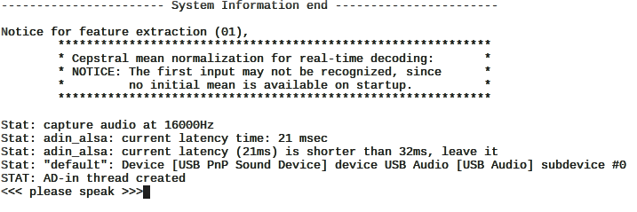
\includegraphics[width=17.006cm,height=5.657cm]{text06-img/text06-img009.png} \newline
juliusの使い方}
\label{seq:refIllustration9}

%\end{figure}
{\selectlanguage{english}
\ \ りんご みかん ぶどう もも あけび あんず いちご いちじく かき スイカ すもも \ \ なし メロン}

{\selectlanguage{english}
終了するときはCtrl+c(コントロールキーを押しながらcを押す)を使います。{\textless}{\textless}please
speak{\textgreater}{\textgreater}と表示されなくなり、pi@raspberrypi:と表示されればOKです。}

{\selectlanguage{english}
Juliusはうまく言葉を認識してくれましたか?おそらく、何度か間違えて認識したと思います。日本語には数多の単語がありますし、似た発音の単語もあるので、それらを完璧に認識することは難しいのです。これを解決するために、「単語辞書」を登録してみましょう。}

{\bfseries
問題6-7}

{\selectlanguage{english}
ターミナルにrun-linux-gmm.shと入力し、Juliusを試してみましょう。\newline
{\textless}{\textless}please
speak{\textgreater}{\textgreater}と表示されたらマイクに向かって果物の名前を5つ話しかけましょう。\newline
何個認識されましたか?}

{\raggedleft\selectlanguage{english}
%\newline
\ \ \ \ 答え\_\_\_\_\_\_\_\_\_\_\_\_\_\_\_\_\_\_\_\_\_\_\_\_\_\_\_\_\_\_\_\_\_\_\_\_\_\_\_\_\_\_\_\_\_\_\_\_\_\_\_\_\_\_\_\_\_\_\_\_\_\_\_
\par}

\subsection{ディレクトリの移動}
{\selectlanguage{english}
Juliusを使ったサンプルプログラムや必要なファイルは/home/pi/ome/06/に用意してあります。ホームディレクトリで作業してもいいですが、入力する引数を短くするためにディレクトリを移動しておきましょう。}

{\bfseries
問題6-8}

\liststyleLxi
\begin{enumerate}
\item {\selectlanguage{english}
ターミナルを開いて、/home/pi/ome/06/に移動しましょう。\newline
ヒント:cd /home/pi/ome/06/\newline
${\square}\leftarrow
できたらチェックしましょう。$}
\end{enumerate}
\subsection[単語辞書]{単語辞書}
\subsubsection[単語辞書を使った音声認識を体験する]{単語辞書を使った音声認識を体験する}
{\selectlanguage{english}
さきほど書いたように、日本語の全ての言葉を認識させるのはとても難しいことです。しかし、多くの場合、認識させたい単語はいくつかに限られる多いです(たとえば、声で操作する照明の場合、「つけて」と「けして」の単語を登録しておけば十分です)。認識させる単語を減らせば、似た発音の単語も減りますし、探索する量も減り、認識の正確さと速度が向上します。ここではJuliusに単語辞書を登録し、その辞書に登録されている単語だけを認識させる方法を紹介します。}

{\selectlanguage{english}
少ない単語を登録した単語辞書をJuliusに読み込ませたときの動作を確認しましょう。juliusで辞書ファイルを使うには、辞書ファイルを引数にして、julius.sh命令を使います。}

{\ttfamily\bfseries
julius.sh {\textless}辞書ファイル名.dic{\textgreater}}

{\selectlanguage{english}
例えば/home/pi/ome/06/に果物の単語を登録した辞書ファイル、kudamono.dicを用意しています。kudamono.dicに下の単語が登録されています。}

{\selectlanguage{english}
\ \ りんご みかん ぶどう もも あけび あんず いちご いちじく かき スイカ すもも \ \ なし メロン}

{\selectlanguage{english}
単語辞書を使うと、単語辞書なしでやったときよりも正確で高速に動作していると思います。これが単語の種類を制限する効果です。みなさんがjuliusを使って何か作りたいと思ったときは単語辞書を作る方法を使うのがおすすめです。}

{\selectlanguage{english}
問題6-9}

\liststyleLxii
\begin{enumerate}
\item {\selectlanguage{english}
ターミナルにjulius.sh
kudamono.dicと入力して、果物の名前を5個話しかけてみましょう。何個認識されましたか?\newline
}
\end{enumerate}
{\raggedleft\selectlanguage{english}
答え\_\_\_\_\_\_\_\_\_\_\_\_\_\_\_\_\_\_\_\_\_\_\_\_\_\_\_\_\_\_\_\_\_\_\_\_\_\_\_\_\_\_\_\_\_\_\_\_\_\_\_\_\_\_\_\_\_\_\_\_\_\_\_
\par}

\subsubsection{自分の単語辞書を作成する手順}
{\selectlanguage{english}
それでは、実際に自分で単語辞書を作成・登録しましょう。大まかな流れは、まず人間が読める形式で辞書(識別子(コンピュータが使うラベル)と読み方のペア)を作成し、それをJuliusが読める形式に変換し、変換したものをjuliusに読み込ませます。辞書ファイルの例として/home/pi/ome/06/kudamono.yomiがあります。}



%\begin{figure}
\centering
\begin{minipage}{17.006cm}
{\ttfamily\bfseries
りんご りんご}

{\ttfamily\bfseries
みかん みかん}

{\ttfamily\bfseries
ぶどう ぶどう}

{\ttfamily\bfseries
桃 もも}

{\ttfamily\bfseries
あけび あけび}

{\ttfamily\bfseries
あんず \ あんず}

{\ttfamily\bfseries
苺 \ \ \ \ \ いちご}

{\ttfamily\bfseries
いちじく \ \ \ \ \ \ \ いちじく}

{\ttfamily\bfseries
柿 \ \ \ \ \ かき}

{\ttfamily\bfseries
スイカ \ すいか}

{\ttfamily\bfseries
すもも \ すもも}

{\ttfamily\bfseries
なし \ \ \ なし}

{\ttfamily\bfseries
メロン \ めろん}

{\upshape
リスト \stepcounter{List}{\theList}: kudamino.yomi}
\end{minipage}
%\end{figure}
{\selectlanguage{english}
このファイルのように、辞書ファイルは\newline
\textbf{「{\textless}コンピュータが使うラベル{\textgreater}
(}\textbf{半角}\textbf{スペース)
{\textless}読み方(ひらがな){\textgreater} (改行)」}\newline
という形式である必要があります。leafpadなどで新しいファイルを開き、この形式で辞書ファイルを作成・保存してください。次に、この.yomiファイルをJuliusが読めるように.dicファイルに変換します。このために、convert\_yomi.shコマンドが用意してあります。使いかたは}

{\selectlanguage{english}\bfseries
convert\_yomi.sh (辞書ファイルの名前 .yomiファイル)
{\textgreater} (辞書ファイルの名前.dicファイル)}

{\selectlanguage{english}
です。これをターミナルに打ち込みます。例えば、}

{\ttfamily\bfseries
convert\_yomi.sh kudamono.yomi {\textgreater} kudamono.dic}

{\selectlanguage{english}
のように使います。}

{\selectlanguage{english}
.dicファイルができたら、これをJuliusから使ってみましょう。Juliusを起動するためのコマンド
julius.sh が用意してあります。}

{\ttfamily\bfseries
julius.sh {\textless}.dicファイル{\textgreater}}

{\selectlanguage{english}
のように使います。たとえば、}

{\ttfamily\bfseries
julius.sh kudamono.dic}

{\selectlanguage{english}
のように使います。これを実行したら、またマイクに向かって話しかけてみて、言葉が認識されるかを確認してください。終了するときは\pageref{bkm:RefHeadingToc20531017892532}ページで説明したように、Ctrl+c(コントロールキーを押しながらcを押す)を使います。}

{\bfseries
問題6-10}

\liststyleLxiii
\begin{enumerate}
\item {\selectlanguage{english}
kudamono.yomiに好きな果物を3つ追加してみましょう。\newline
${\square}\leftarrow
できたらチェックしましょう。$}
\item {\selectlanguage{english}
辞書ファイルを変換しましょう。\newline
ターミナルにconvert\_yomi.sh kudamono.yomi {\textgreater}
kudamono.dicと入力します。\newline
${\square}\leftarrow
できたらチェックしましょう。$}
\item {\selectlanguage{english}
果物を追加したkudamono.dicで音声認識をしてみましょう。\newline
ターミナルにjulius.sh
kudamono.dicと入力します。\newline
${\square}\leftarrow
追加した果物が認識されたらチェックしましょう。$}
\item {\selectlanguage{english}
時間があったらやりましょう。\newline
3単語以上からなるオリジナル辞書を作成し、juliusに認識させてみましょう。\newline
${\square}\leftarrow
できたらチェックしましょう。$}
\end{enumerate}
\subsection{HSPからJuliusを使う}
{\selectlanguage{english}
認識した音声を元に何か処理を行いたいことはしばしばあります。例えば、認識した音声に応じて部屋の電気をつけたり、タイマーをセットしたりということが考えられます。そんなときには自分のプログラムと連携させましょう。}

\subsubsection[JuliusとHSPの連携のしくみ]{JuliusとHSPの連携のしくみ}
{\selectlanguage{english}
Juliusは図\ref{seq:refIllustration10}のように、HSPの外で動きます。別に起動しているJuliusと、書いたHSPプログラムが「ソケット」と呼ばれる通信経路を介して通信することで認識結果やコマンド(Juliusの起動・停止など)のやり取りをすることができます。}



%\begin{figure}
\centering
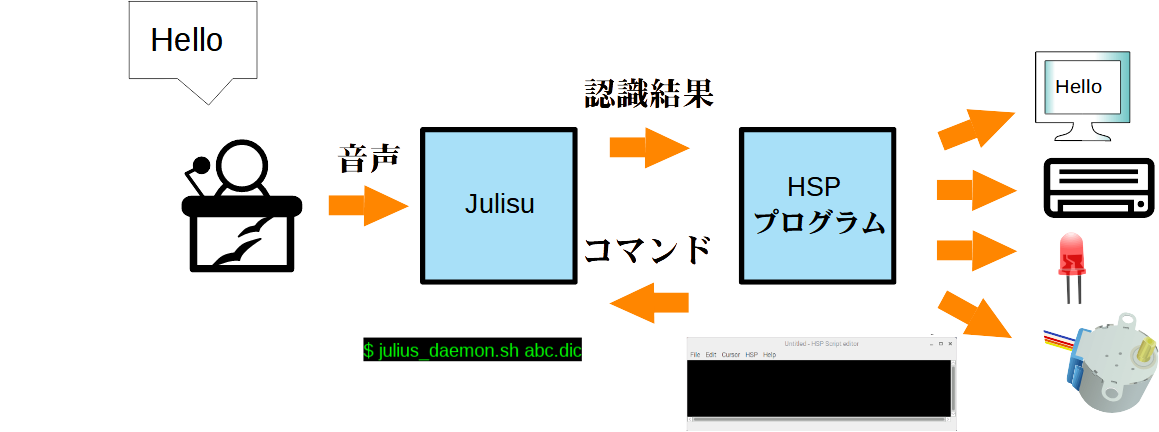
\includegraphics[width=17.006cm,height=6.332cm]{text06-img/text06-img010.png}
\caption[JuliusとHSPの連携]{\newline
JuliusとHSPの連携}
\label{seq:refIllustration10}

%\end{figure}
{\selectlanguage{english}
従って、HSPからJuliusを使うためには、HSPプログラムだけではなく別にJuliusも事前に起動させておかなければなりません。}

\subsubsection{認識した単語を取得・表示する}
{\selectlanguage{english}
新しく覚える命令と関数はinit\_julius, is\_recieved(),
get\_word\_list の3つです。例題のプログラム julius.hsp
を見ながら解説していきます。}



%\begin{figure}
\centering
\begin{minipage}{17.006cm}
{\ttfamily\bfseries
\#include {\textquotedbl}hsp3dish.as{\textquotedbl}}

{\ttfamily\bfseries
\#include {\textquotedbl}julius.as{\textquotedbl}}


\bigskip

{\ttfamily\bfseries
redraw 0}

{\ttfamily\bfseries
pos 0, 0}

{\ttfamily\bfseries
mes {\textquotedbl}Loading Julius...{\textquotedbl}}

{\ttfamily\bfseries
redraw 1}


\bigskip

{\ttfamily\bfseries
init\_julius {\textquotedbl}/home/pi/ome/06/kudamono.dic{\textquotedbl}}


\bigskip

{\ttfamily\bfseries
sockidx = 0}

{\ttfamily\bfseries
domain = {\textquotedbl}127.0.0.1{\textquotedbl}}

{\ttfamily\bfseries
PORT = 10500}


\bigskip

{\ttfamily\bfseries
sockopen sockidx, domain, PORT}


\bigskip

{\ttfamily\bfseries
if stat != 0 \{}

{\ttfamily\bfseries
*errorjulius}

{\ttfamily\bfseries
\ \ redraw 0}

{\ttfamily\bfseries
\ \ pos 0, 0}

{\ttfamily\bfseries
\ \ mes {\textquotedbl}Error in opening socket{\textquotedbl}}

{\ttfamily\bfseries
\ \ redraw 1}

{\ttfamily\bfseries
\ \ await 30}

{\ttfamily\bfseries
\ \ goto *errorjulius}

{\ttfamily\bfseries
\ \ stop}

{\ttfamily\bfseries
\}}


\bigskip

{\ttfamily\bfseries
sdim words, 4096, 0}

{\ttfamily\bfseries
ddim cm, 0}


\bigskip

{\ttfamily\bfseries
repeat -1}

{\ttfamily\bfseries
\ \ if is\_recieved(sockidx) == 0 \{}

{\ttfamily\bfseries
\ \ \ \ get\_word\_list words, cm}

{\ttfamily\bfseries
\ \ \ \ len = \ {\textquotedbl}L1 {\textquotedbl} + length(words)}

{\ttfamily\bfseries
\ \ \ \ repeat length(words)}

{\ttfamily\bfseries
\ \ \ \ \ \ if cm(cnt) {\textgreater} 0.5 \{}

{\ttfamily\bfseries
\ \ \ \ \ \ \ \ \ \ ans = \ {\textquotedbl}{\textquotedbl} + cnt + {\textquotedbl}: {\textquotedbl} + words(cnt) +
{\textquotedbl} CM = {\textquotedbl} + cm(cnt)}

{\ttfamily\bfseries
\ \ \ \ \ \ \}}

{\ttfamily\bfseries
\ \ \ \ loop}

{\ttfamily\bfseries
\ \ \}}

{\ttfamily\bfseries
\ \ redraw 0}

{\ttfamily\bfseries
\ \ pos 0,0}

{\ttfamily\bfseries
\ \ mes len}

{\ttfamily\bfseries
\ \ mes ans}

{\ttfamily\bfseries
\ \ redraw 1}

{\ttfamily\bfseries
\ \ await 30}

{\ttfamily\bfseries
loop}

{\upshape
リスト \stepcounter{List}{\theList}: julius.hsp}
\end{minipage}
%\end{figure}
{\selectlanguage{english}
まず、init\_julius,is\_recievedとget\_word\_listを使えるようにするために、2行目のように}

{\ttfamily\bfseries
\#include ``julius.as{}''}

{\selectlanguage{english}
を書きます。}

{\selectlanguage{english}
続いて、init\_juliusを実行してjuliusを使うための初期化
(initialization)
を行います。これはis\_recievedとget\_word\_listが実行される前に一回だけ実行されるよう書く必要があります。これによってJuliusが起動します。引数には使用する辞書ファイル
(今回は\texttt{/home/pi/ome/06/kudamono.dic})
を指定してください。続いて、sockopen命令でjuliusと通信するための経路
の番号(ソケットIDと呼びます)
をsockidx、つまり0に設定します。juliusは自分のラズベリーパイ
(127.0.0.1)
の10500番ポートを使用します。このとき、エラーが起きればシステム変数statに0以外の値が入るので、statに0以外の値が入っていたらエラーメッセージを表示して終了する条件分岐を書きます。}

{\selectlanguage{english}
続いて、}

{\ttfamily\bfseries
sdim words, 4096, 0}

{\ttfamily\bfseries
ddim cm, 0}

{\selectlanguage{english}
は、juliusの認識結果を格納するための配列を宣言しています。juliusは認識結果として2つの要素を出力します:
1つめは認識された単語、2つ目は認識の正確さ(単語信頼度)です。それぞれが文字列配列wordと小数配列cmに格納されます。認識された単語が必要なのはもっともですね。単語信頼度は、juliusがその認識結果にどれだけ自信があるかを示します。1が最大(最も自信がある)で0が最小(最も自信がない)で、小数で表されます。}

{\ttfamily\bfseries
repeat -1}

{\selectlanguage{english}
以下が認識結果を画面に表示するための無限ループによるメインルーチンになります。is\_recieved(sockidx)は、sockidxの先のjuliusから認識結果を取得し終えたら0が帰ってきます。従って、0が返ってきたときだけ認識結果の代入と画面表示の処理を行うように条件分岐が書いてあります。}

{\ttfamily\bfseries
get\_word\_list word, cm}

{\selectlanguage{english}
によって、文字列配列wordと小数配列cmに認識結果が代入されます。wordとcmは配列なので、次のrepeat文でそれぞれの要素に対して、cm(単語信頼度)が0.5以上のもののみmes命令を実行し、結果を画面に表示させています。}

{\bfseries
問題6-11}

\liststyleLxiv
\begin{enumerate}
\item {\selectlanguage{english}
HSPでjulius.hspを実行しましょう。\newline
果物の名前を3つ話しかけて、認識されるか確かめてみましょう。\newline
${\square}\leftarrow
できたらチェックしましょう。$}
\end{enumerate}
\subsection{Juliusが起動しなくなったら}
{\selectlanguage{english}
もしもJuliusがうまく起動しなくなったときは、インストールしてあるコマンド}

{\ttfamily\bfseries
stopjulius.sh}


\bigskip

{\selectlanguage{english}
を一度実行してからもう一度起動を試してみましょう。このコマンドは、上手く終了できなかった前のJuliusを終了させるコマンドです。}

\subsection{音声でLEDのON OFFをする}
{\selectlanguage{english}
HSPプログラムから、音声を使ってLEDをつけたり消したりしてみましょう。/home/pi/ome/06にonoff.yomiファイルがあります。これは音声でLEDのON/OFFをするための辞書ファイルです\newline
\begin{minipage}{17.006cm}
{\ttfamily\bfseries
ON おん}

{\ttfamily\bfseries
OFF おふ}

{\upshape
リスト {\refstepcounter{List}\theList\label{seq:refList6}}: onoff.yomi}
\end{minipage}}

{\selectlanguage{english}
リスト 7:
onoff.yomiのように書いてあります。ONとOFFが表示する文字、おんとおふが読み方です。これをconvert\_yomi.shを使って変換したものがonoff.dicです。onoff.dicを使って、音声からLEDを制御してみましょう。/home/pi/ome/06/ledbyvoice.hsp
を開いてください。}



%\begin{figure}
\centering
\begin{minipage}{17.006cm}
{\ttfamily\bfseries
\#include {\textquotedbl}hsp3dish.as{\textquotedbl}\newline
\#include {\textquotedbl}julius.as{\textquotedbl}\newline
\newline
redraw 0}

\begin{minipage}{16.621cm}
{\ttfamily\bfseries
\ \ \ \ \ \ \ \   if words(cnt) = {\textquotedbl}ON{\textquotedbl} \{\ \ \ \ 
\textcolor[rgb]{0.0,0.0,0.6}{;認識された文字がONのとき}}

{\ttfamily\bfseries
\ \ \ \ \ \ \ \ \ \ \ \ \ \ gpio 17, 1\ \ \ \ \ \ \ \ 
\textcolor[rgb]{0.0,0.0,0.6}{;GPIO17のLEDを光らせる}}

{\ttfamily\bfseries
\ \ \ \ \ \ \ \ \ \ \}else : if words(cnt) = {\textquotedbl}OFF{\textquotedbl} \{\ \ 
\textcolor[rgb]{0.0,0.0,0.6}{;認識された文字がOFFのとき}}

{\ttfamily\bfseries
\ \ \ \ \ \ \ \ \ \ \ \ \ \ gpio 17, 0\ \ \ \ \ \ \ \  \textcolor[rgb]{0.0,0.0,0.6}{;GPIO17を消す}}

{\ttfamily\bfseries
\ \ \ \ \ \ \ \ \ \ \}}
\end{minipage}{\ttfamily\bfseries
pos 0, 0}

{\ttfamily\bfseries
mes {\textquotedbl}Loading Julius...{\textquotedbl}}

{\ttfamily\bfseries
redraw 1}


\bigskip

{\ttfamily\bfseries
init\_julius {\textquotedbl}/home/pi/ome/06/onoff.dic{\textquotedbl}\newline
\newline
sockidx = 0\newline
domain = {\textquotedbl}127.0.0.1{\textquotedbl}\newline
PORT = 10500\newline
\newline
sockopen sockidx, domain, PORT\newline
\newline
if stat != 0 \{\newline
 \ redraw 0\newline
 \ mes {\textquotedbl}Error in opening socket{\textquotedbl}\newline
 \ redraw 1\newline
 \ wait 30\newline
 \ stop\newline
\}\newline
\newline
sdim wrods, 4096, 0\newline
ddim cm, 0\newline
repeat -1\newline
 \ redraw 0\newline
 \ if is\_recieved(sockidx) = 0 \{\newline
 \ \ \ get\_word\_list words, cm\newline
 \ \ \ repeat length(words)\newline
 \ \ \ \ \ if cm(cnt) {\textgreater} 0.7 \{\newline
 \ \ \ \ \ \} \ \ }

{\ttfamily\bfseries
 loop\newline
 \ \}\newline
 \ redraw 0\newline
 \ pos 0,0\newline
 \ mes
{\textquotedbl}話しかけてLEDのONとOFFをしよう{\textquotedbl}\newline
 \ redraw 1\newline
 \ await 30\newline
loop\newline
}
\end{minipage}
%\end{figure}
{\selectlanguage{english}
words(cnt)に認識された文字が代入されています。認識された文字がONなのかOFFかif文(条件分岐)を使って、LEDを制御しています。}

{\bfseries
問題6-12}

\liststyleLxv
\begin{enumerate}
\item
ledbyvoice.hspをHSPスクリプトエディタで実行しましょう。\newline
${\square}\leftarrow
オン、オフと話しかけて$LEDをつけたり消したりできたらチェックしましょう。
\item 点灯させるLEDを変更しましょう。\newline
${\square}\leftarrow できたらチェックしましょう。$
\item 時間があったらやりましょう。\newline
点灯させるための言葉を「つける」と「けす」に変更しましょう。\newline
${\square}\leftarrow できたらチェックしましょう。$
\item 時間があったらやりましょう。\newline
センサーボードには4色のLEDが点いています。色ONでその色のLEDがつき、色OFFでその色のLEDが消えるようなプログラムを書きましょう。(オレンジONでオレンジ色のLEDがつき、オレンジOFFでオレンジ色のLEDが消えるなど)\newline
${\square}\leftarrow できたらチェックしましょう。$
\end{enumerate}
\subsection[文法を設定する(発展)]{文法を設定する(発展)}
{\selectlanguage{english}
例えば数字を認識させたいときはどうすればよいでしょうか?実はこれを単語辞書のみで実現するとなると大変な労力が必要です。例えば123という数をするには、単語辞書のみを使う場合は「ひゃくにじゅうさん」という単語を登録しないといけません。そうしなければ「いちにさん」と読まれてしまいます。同様に、それぞれの数に対して読みを登録しておかないといけません。また、同じ数字でも読み方が違う場合もあります(例えば、7は「なな」や「しち」と読むことがあります)。つまり、1から1000までの数を認識させたいときは、1000個以上の単語を登録しなければなりません。これを解決するために、「文法」を定めることができます。ただ、これは難しいので、興味があれば以下のページなどを参考に挑戦してみてください。}

\liststyleLxvi
\begin{itemize}
\item {\selectlanguage{english}
\url{http://www.atmarkit.co.jp/fxml/ddd/ddd004/ddd004-bnf.html} }
\item {\selectlanguage{english}
\href{http://julius.osdn.jp/index.php?q=doc/grammar.html}{http://julius.osdn.jp/index.php?q=doc/grammar.htm}\href{http://julius.osdn.jp/index.php?q=doc/grammar.html}{l}}
\end{itemize}
\section{まとめ}
{\selectlanguage{english}
OpenJTalkとJuliusの使いかたをまとめました。OpenJtalkの使いかたは、HSPスクリプトエディタで}

{\ttfamily\bfseries
jtload ``{\textless}読み上げたい文字列{\textgreater}'',
{\textless}バッファ番号{\textgreater}}

{\selectlanguage{english}
で音声をロードした後、}

{\ttfamily\bfseries
mmplay {\textless}バッファ番号{\textgreater}}


\bigskip

{\selectlanguage{english}
Juliusはターミナルで使うときは}

{\ttfamily\bfseries
julius.sh {\textless}.dicファイル{\textgreater}}

{\selectlanguage{english}
のように使います。dic形式の辞書は、.yomiファイル
(識別子(コンピュータが使うラベル)と読み方のペア)
を作って、ターミナルに\ \ }

{\ttfamily\bfseries
convert\_yomi.sh (今作った.yomiファイル) {\textgreater}
(出力するファイルの名前(.dicファイル))}

{\selectlanguage{english}
とします。}

{\selectlanguage{english}
HSPから使うときはinit\_julius, is\_received, get\_word\_list
を使って認識結果を取得します。}

{\selectlanguage{english}
init\_julius {\textless}dicファイル{\textgreater}}

{\selectlanguage{english}
で辞書ファイルをしつつJuliusを初期化します。}

{\selectlanguage{english}
is\_received {\textless}ソケットID{\textgreater}}

{\selectlanguage{english}
でJuliusが単語を受信したかチェックします。}

{\selectlanguage{english}
get\_word\_list
{\textless}単語をあらわす文字列配列{\textgreater}
{\textless}単語信頼度をあらわす小数配列{\textgreater}}

{\selectlanguage{english}
は、is\_received
{\textless}単語をあらわす文字列配列{\textgreater}
{\textless}単語信頼度をあらわす小数配列{\textgreater}}

\section{宿題}
{\selectlanguage{english}
この中から好きな問題を1つ以上選んで、プログラムを作ってみましょう。}

\liststyleLxvii
\begin{enumerate}
\item {\selectlanguage{english}
HSPで以下のようなプログラムを書きましょう。まず数字
(0から9まで)
のキー入力を受け付けます。キーが押されたらすぐにその数字をOpenJTalkに読み上げさせます。例えば、4キーが押されたら「よん」と読み上げさせます。}
\item {\selectlanguage{english}
HSPで以下のようなプログラムを書きましょう。数字(0から9まで)のキーとエンターキーの入力を受け付けます。エンターキーが押されたら、プログラム開始後または直前にエンターキーが押されたあとに押された数字を順番に全て読み上げさせます。たとえば、
[1, 2, エンターキー, 5, 0,
エンターキー]とキーが押されたら、最初にエンターキーが押されたときに「いち に」と、2番めのエンターキーがおされたら「ご ぜろ」と読み上げさせます。}
\item {\selectlanguage{english}
HSPで以下のようなプログラムを書きましょう。異なる種類の画像を3枚用意します(例:車の画像、犬の画像、時計の画像)。これを画面に並べて表示します。どれかの画像がクリックされたら、直ちにその画像に写っているものを読み上げさせます。例えば、車の画像がクリックされたら「くるま」と読み上げさせます。}
\item {\selectlanguage{english}
HSPで、文字の色を声で変えるプログラムを作りましょう。まず、画面に文字を表示します。例えば、「こんにちは」を表示しておきます。はじめの色は何色でも構いません。「あお」、「あか」、「きいろ」という音声を受け付けます。もし、「あお」という声が入力されたら、文字の色を青色にします。もし、「あか」という声が入力されたら、文字の色を赤色にします。もし、「きいろ」という声が入力されたら、文字の色を黄色にします。}
\item {\selectlanguage{english}
HSPで以下のようなプログラムを書きましょう。異なる種類の画像を3枚用意します。初めは何も画面に表示しません。今用意した3種類の画像を表す声を受け付けます。声が入力されたら、その声が表す画像だけを表示させます。例えば、
車の画像、犬の画像、時計の画像を用意します。もし「くるま」という声を入力したら、画面に車の画像を表示します。他の画像は表示しません。以下同様にします。}
\end{enumerate}
\section{参考文献}
\liststyleLxviii
\begin{itemize}
\item {\selectlanguage{english}
おにたま, 悠黒喧史, うすあじ.
HSPでつくる! はじめてのプログラミング
HSP3.5+3Dish入門. 秀和システム. 2017}
\end{itemize}
{\selectlanguage{english}
OpenJtalkについて}

\liststyleLxix
\begin{itemize}
\item {\selectlanguage{english}
Open JTalk - HMM-based Text-to-Speech System\newline
\href{http://open-jtalk.sp.nitech.ac.jp/}{http://open-}\href{http://open-jtalk.sp.nitech.ac.jp/}{jtalk.sp.nitech.ac.jp/}}
\item {\selectlanguage{english}
Open JTalk
(テキストを音声へ変換)をインストールし、使ってみる~{\textbar}~レンタルサーバー・自宅サーバー設定・構築のヒント\newline
\url{https://server-setting.info/centos/open-jtalk-install.html}}
\end{itemize}
{\selectlanguage{english}
Juliusについて}

\liststyleLxx
\begin{itemize}
\item {\selectlanguage{english}
大語彙連続音声認識エンジン Julius\newline
\url{http://julius.osdn.jp/}}
\end{itemize}
\end{document}
